\chapter{Model Validation}
\label{chp:MV}

%%%%%%%%%%%%%%%%%%%%%%%%%%%%%%%%%%%%%%%%%%%%%%%%%%%%%%%%%%%%%%%%%%%%%%%

Physical replicas of selected units are constructed and inflated. The deformation is observed and compared with the modelled behaviour as calculated by the FEM software.

\section{FEM}

FEM models were adapted for model validation. Only a single unit was manufactured at a time. Units were modelled and manufactured with $\SI{1}{cm}\times \SI{1}{cm}$ sized elements. Constructing a $5\times 5$ grid of the unit is impractical at the current scale. FEM models selected for model validation were adjusted accordingly. Surrounding units were removed. A fixed displacement boundary condition was applied to the bottom left node of the unit. Figure~ illustrates the boundary conditions as applied to grid\_.

\section{Mixing and Casting}

The modular mould as described in Section~\ref{ssec:pc} is assembled according to the desired unit layout. Mold Star 15 is mixed and cast as per Section~\ref{ssec:mac}. Figure~\ref{fig:fillmould} shows a filled mould. After the cure time has passed the unit is removed from the mould and excess material is carefully cut off. 

\begin{figure}[H]
	\centering
	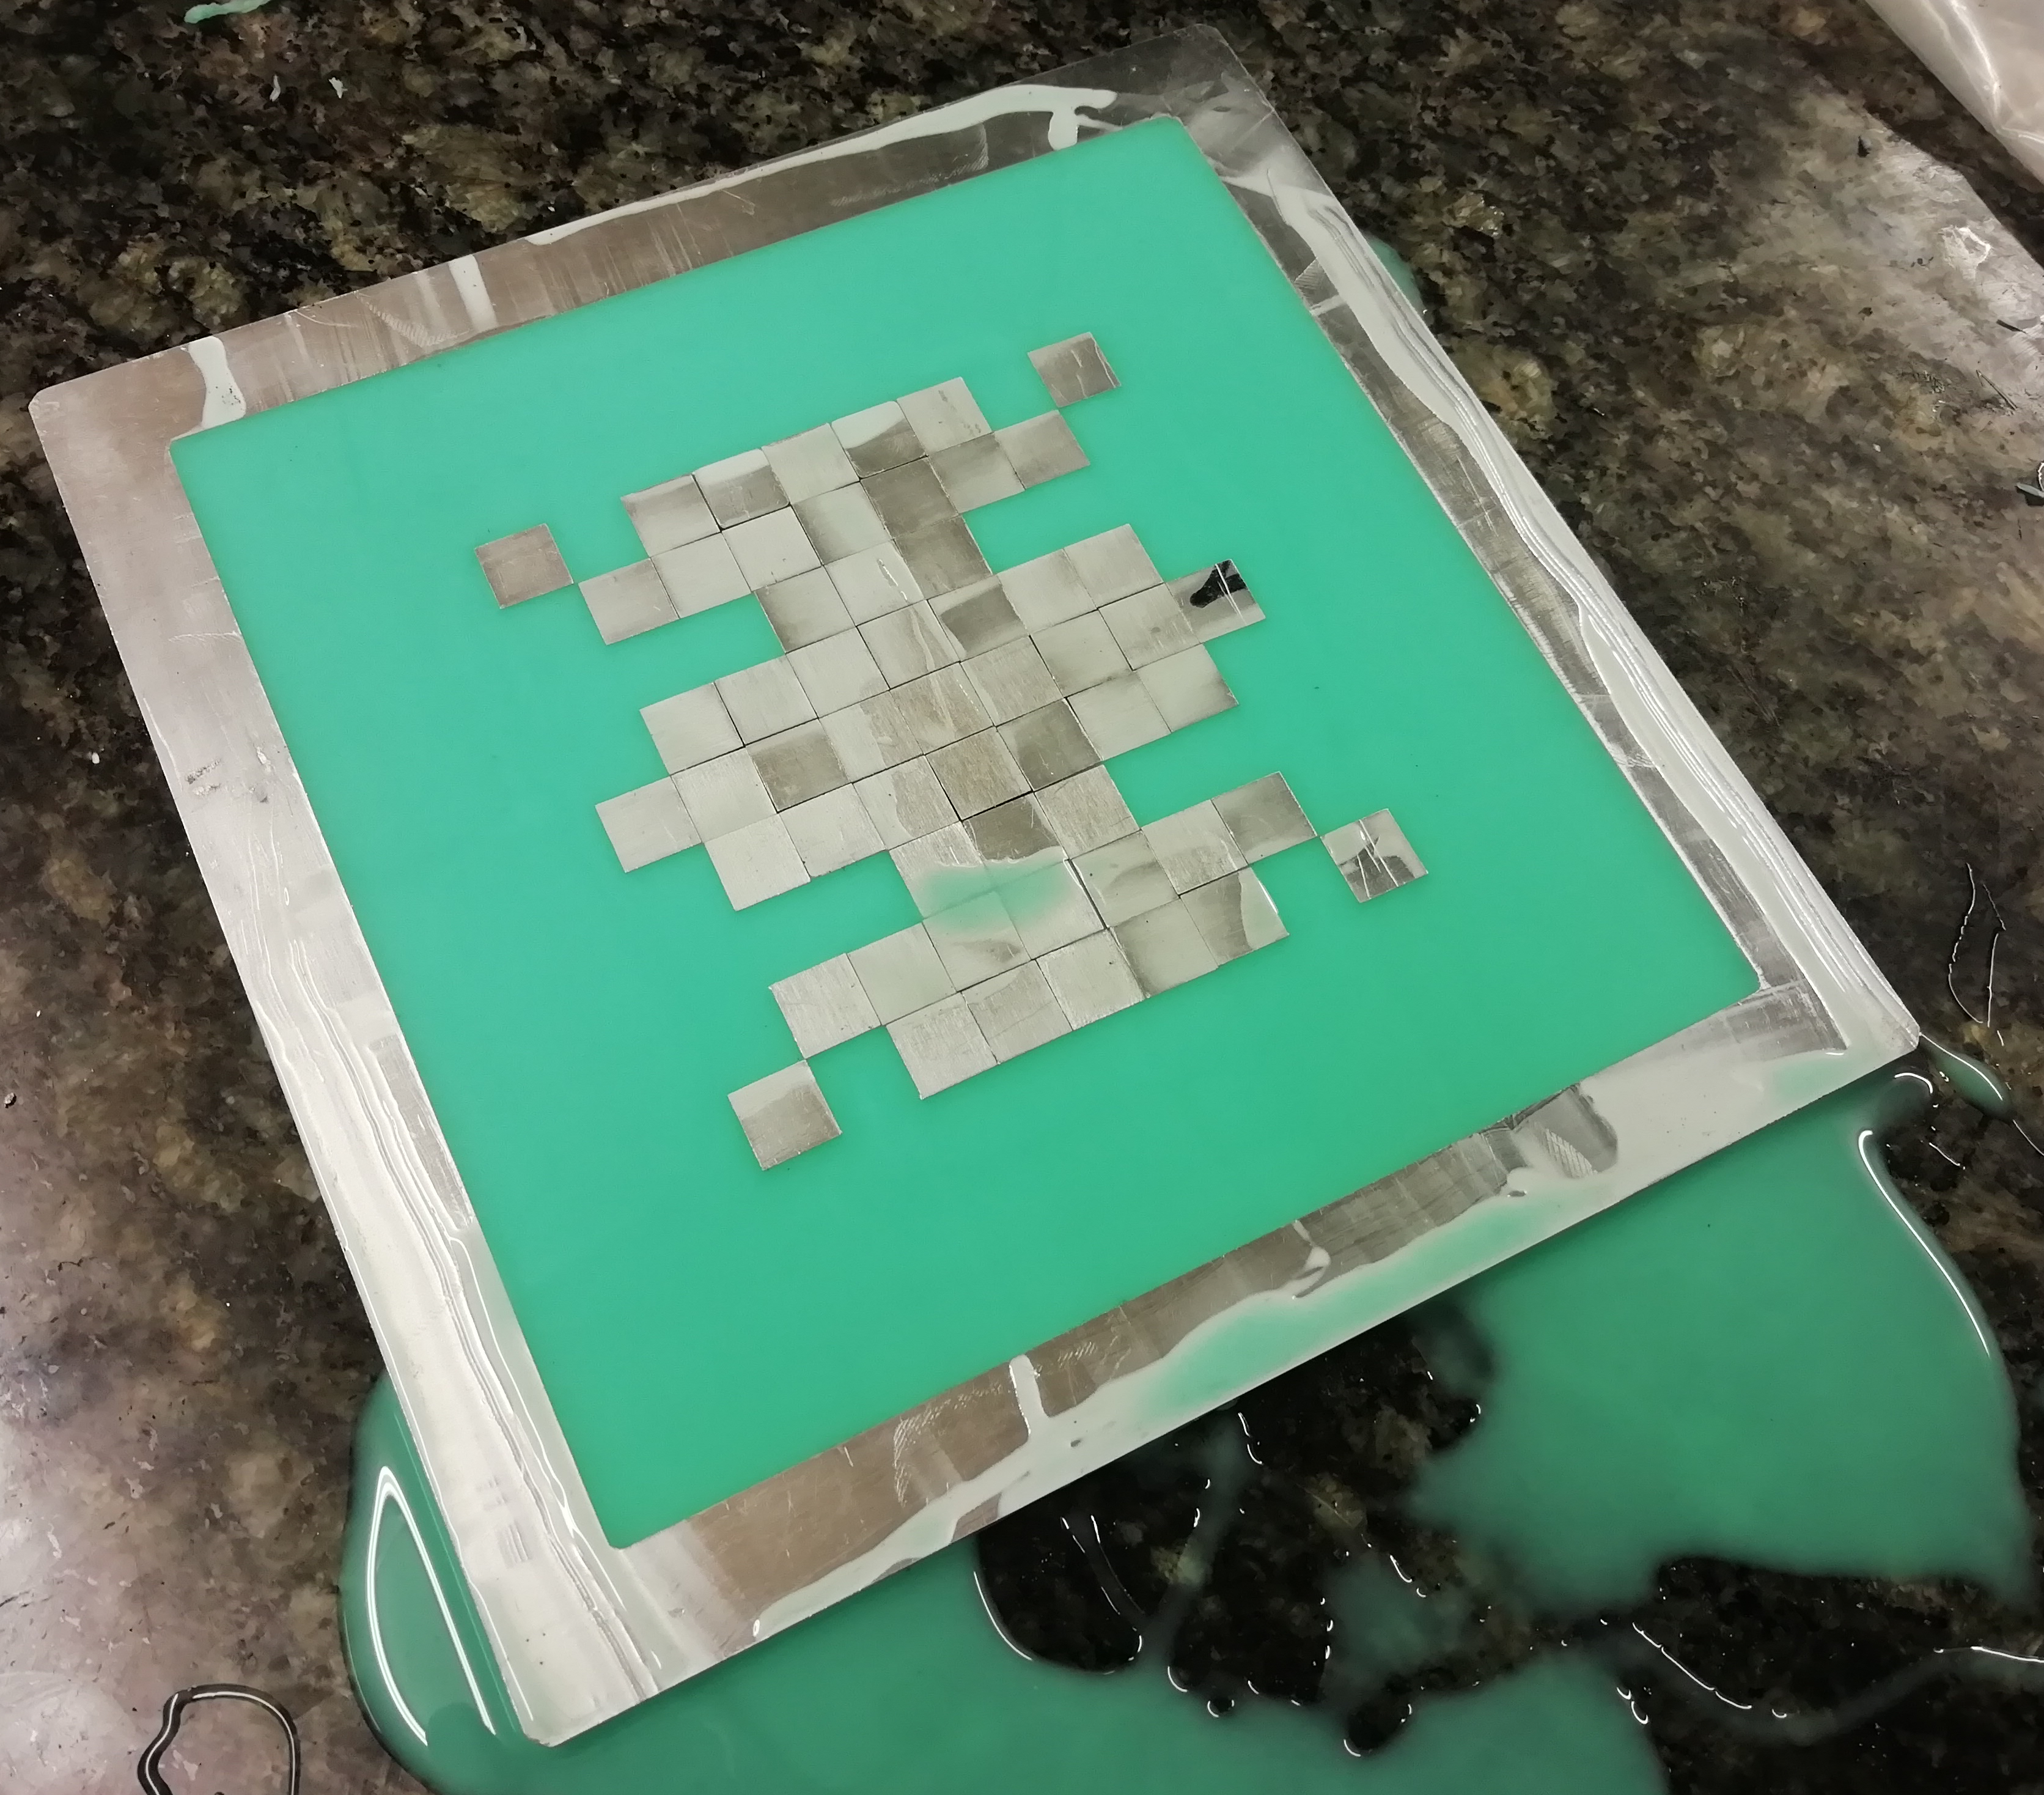
\includegraphics[width=0.5\textwidth]{MouldFilled.png}
	\caption[A filled unit mould]{A unit mould filled with Mold Star 15 before it has cured. Excess material that has been removed is visible around the mould.}
	\label{fig:fillmould}
\end{figure}

\section{Experimental Setup}

The experimental setup as described in Section~\ref{ssec:pc} is constructed. Figure~\ref{fig:expempty} shows the experimental setup with no unit in place.

\begin{figure}[H]
	\centering
	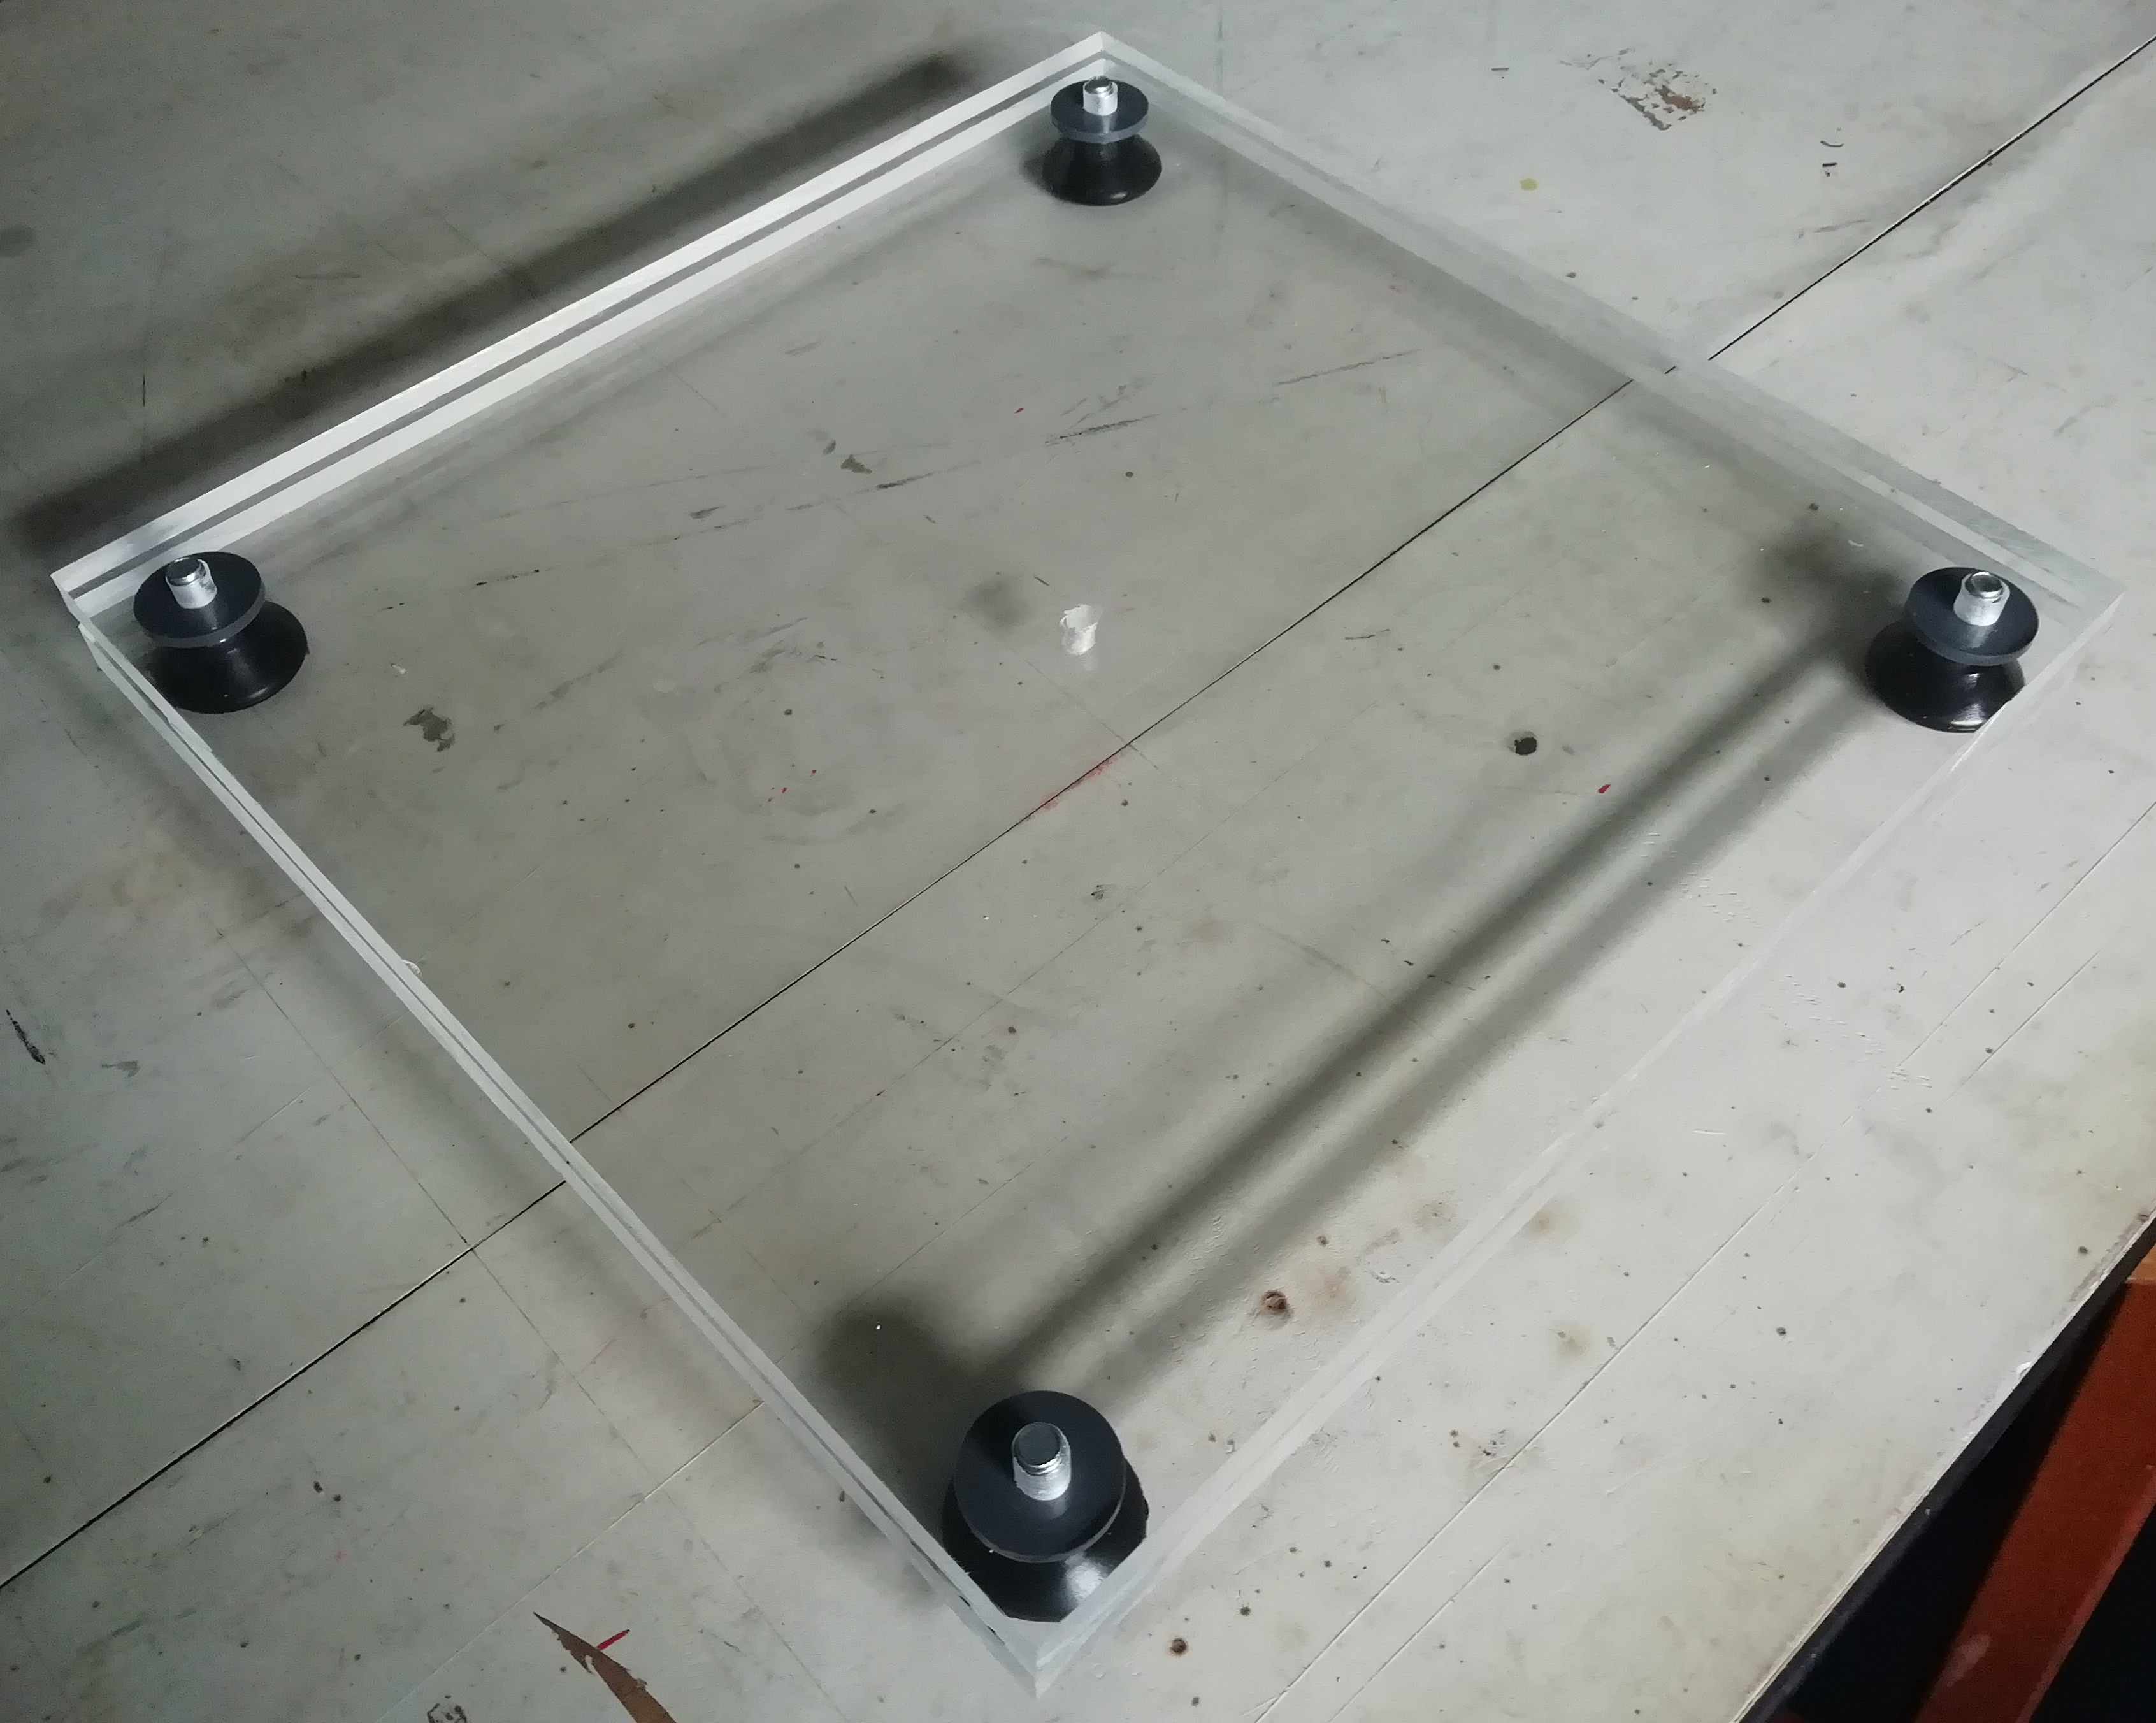
\includegraphics[width=0.5\textwidth]{rig_empty.png}
	\caption[The experimental setup without a unit]{The experimental setup with no unit in place and the pressure hose unconnected}
	\label{fig:expempty}
\end{figure}

The pressure hose is inserted into the hole in the bottom plate. A sealant is applied to prevent air leakage at the point of entry of the pressure hose.

\section{Results}

Three units were selected for model validation.

\subsection{Unit 1}

The first unit selected is grid\_36\_d68df4e04590e068b46c0e75dcdf5818. This unit was selected as a random control unit. This unit does not perform well according to any specific unit deformation case. This unit has complex internal geometry that may deform in unusual ways. Cavities exist which are potentially inaccessible from the undeformed state, but become accessible as the unit inflates. An additional cavity exists which is not accessible with the experimental setup. This was replicated in the FEM model. The FEM model with boundary conditions is illustrated in Figure~\ref{fig:unit1bc}. The physical model is illustrated in Figure~.

\begin{figure}[H]
	\centering
	\includegraphics[width=0.5\textwidth]{unit1bc.png}
	\caption[FEM validation model of unit 1]{grid\_36\_d68df4e04590e068b46c0e75dcdf5818 FEM model with applied boundary conditions}
	\label{fig:unit1bc}
\end{figure}

Figure~\ref{fig:unit1def} shows comparisons between the FEM model and the physical model as the internal pressure is increased.

\begin{figure}[H]
	\centering
	\begin{subfigure}[c]{\textwidth}
		\centering
		\includegraphics[width=\textwidth]{unit1deffem.png}
		\caption{FEM model deformation as internal pressure is increased}
	\end{subfigure}
	\hfill
	\begin{subfigure}[c]{\textwidth}
		\centering
		\includegraphics[width=\textwidth]{unit1defmod.png}
		\caption{Physical model deformation as internal pressure is increased}
	\end{subfigure}
	\caption[Comparison between FEM and physical models of unit 1]{Comparison between deformation of the FEM model and physical model of grid\_36\_d68df4e04590e068b46c0e75dcdf5818 as the internal pressure is increased}
	\label{fig:unit1def}
\end{figure}

\subsection{Unit 2}

The second unit selected is grid\_ as illustrated in Figure~. This unit was selected as a linearly extending unit. This unit performs well according to the uniaxial deformation case. Cavities exist which are potentially inaccessible from the undeformed state, but become accessible as the unit inflates.

\subsection{Unit 3}

The third unit selected is grid\_ as illustrated in Figure~. This unit was selected as a linearly extending unit. This unit performs well according to the uniaxial deformation case when surrounded by identical units, but performs poorly when on its own.

\section{Issues Encountered}

Issues were encountered during model validation. Some were attempted to account for beforehand and some were unforeseen.

Mould cells were not manufactured exactly to tolerances.